\documentclass[12pt]{article}
\usepackage[utf8]{inputenc}
\usepackage{graphicx}
\usepackage{amsmath}
\usepackage{color}
\title{Producto 7 : Análisis de Mareas.}
\author{Olga María Fimbres Morales}
\date{}
\begin{document}
\maketitle



\begin{large}
La marea es el cambio periódico del nivel del mar producido principalmente por la fuerza de atracción gravitatoria que ejercen el Sol y la Luna sobre la Tierra.\\ 
\\Aunque dicha atracción se ejerce sobre todo el planeta, tanto en su parte sólida como líquida y gaseosa, principalmente se habla sobre la atracción de la Luna y el Sol, juntos o por separado, sobre las aguas de los mares y océanos.\\
\\Sin embargo, hay que indicar que las mareas de la litosfera son prácticamente insignificantes, con respecto a las que ocurren en el mar u océano (que pueden modificar su nivel en varios metros) y, sobre todo, en la atmósfera, donde puede variar en varios km de altura, aunque en este caso, es mucho mayor el aumento del espesor de la atmósfera producido por la fuerza centrífuga del movimiento de rotación en la zona ecuatorial (donde el espesor de la atmósfera es mucho mayor) que la modificación introducida por las mareas en dicha zona ecuatorial.
\\
\\Otros fenómenos ocasionales, como los vientos, las lluvias, el desborde de ríos y los tsunamis provocan variaciones del nivel del mar, también ocasionales, pero no pueden ser calificados de mareas, pero que no están causados por la fuerza gravitatoria.\\
\end{large}

\newpage
\begin{center}
\begin{LARGE}
Historia de las mareas.
\end{LARGE}
\end{center}

\begin{large}
El fenómeno de las mareas es conocido desde la antigüedad.\\Parece ser que Piteas (siglo IV a. C.) fue el primero en señalar la relación entre la amplitud de la marea y las fases de la Luna, así como su periodicidad. Plinio el Viejo (23-79) en su Naturalis Historia describe correctamente el fenómeno y piensa que la marea está relacionada con la Luna y el Sol. \\Mucho más tarde, Bacon, Kepler y otros trataron de explicar ese fenómeno, admitiendo la atracción de la Luna y del Sol. Pero fue Isaac Newton en su obra Philosophiae Naturalis Principia Mathematica («Principios matemáticos de la Filosofía Natural», 1687) quien dio la explicación de las mareas aceptada actualmente. Más tarde, Pierre-Simon Laplace (1749-1827) y otros científicos ampliaron el estudio de las mareas desde un punto de vista dinámico.\\
\\
Isaac Newton realizó varios estudios científicos del comportamiento de las mareas y calculó la altura de éstas según la fecha del mes, la estación del año y la latitud. Más tarde, Simon Laplace complementó los estudios de Newton.
\end{large} 
 
\begin{center}
\begin{LARGE}
Tipos de mareas.
\end{LARGE}
\end{center}
\begin{large}
Según la geografía del lugar y el tipo de vientos predominantes:\\
\\- Semidiurnas: es el tipo de mareas del Río de la Plata, hay dos pleas y dos bajas, en el transcurso de un día lunar. En el caso específico del Río de la Plata de desigualdades diurnas por no ser coincidentes los valores de las dos pleamares entre sí ni de las dos bajamares. Considerando que el día lunar tiene una duración de 24 h 50 min, teóricamente cada 6 h 13 min se produce una pleamar o una bajamar.\\
\\-Diurnas: características en las latitudes bajas, con una pleamar y una bajamar en el transcurso del día lunar. Considerando que el día lunar es de 24 h 50 min se producirá una pleamar y una bajamar cada 12 h 25 min.\\
\\-Diurnas irregulares: con dos ciclos por día lunar pero con marcadas diferencias en las alturas y en los períodos de tiempo.\\
\\-Mareas mixtas: régimen de tipo intermedio, durante un día lunar se presentan dos pleamares y una bajamar o dos bajamares y una pleamar.

\end{large}
\begin{center}
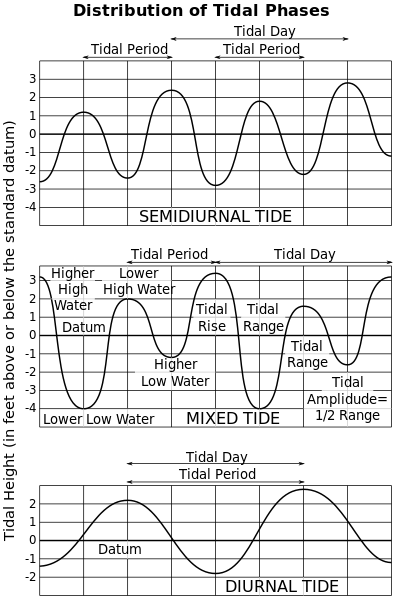
\includegraphics[scale=0.6]{Tide_type.png}  
\end{center}


\newpage
\begin{center}
\begin{LARGE}
Descripción de la actividad.
\end{LARGE}
\end{center}

\begin{large}
La actividad que se realizó consisita en analizar un documento que contenia los datos de los niveles de marea del manglar "El Sargento". Los datos consisten en fecha, hora, presión, temperatura y nivel de las mareas de aproximadamente 5 meses; registrando un dato nuevo cada media hora.\\
\\
Una vez leido el archivo, debia de obtenerse los niveles de las mareas m\'{a}ximos para cada mes y la diferencia de tiempo con que estas ocurrian y asi obtener el periodo del ciclo lunar de las mareas.\\
\\
De igual modo debian obtenerse las mareas m\'{a}ximas en lapsos de 24 horas y en lapsos de 12 horas con su respectivo perioro, para obtener asi los periodos de las mareas diurnas y semidiurnas respectivamente.\\
\\
\end{large}

\newpage
\begin{center}
\begin{LARGE}
Evidencias y conclusiones.
\end{LARGE}
\end{center}

\begin{large}
Mareas diurnas.\\
Al realizar el analisis de las mareas buscando un máximo y un mínimo cada 24 horas se encontro que el periodo entre cada marea diurna fue de aproximadamente de 1.0015 dias, o bien de 24 horas y 2 minutos.
\end{large}
\begin{center}
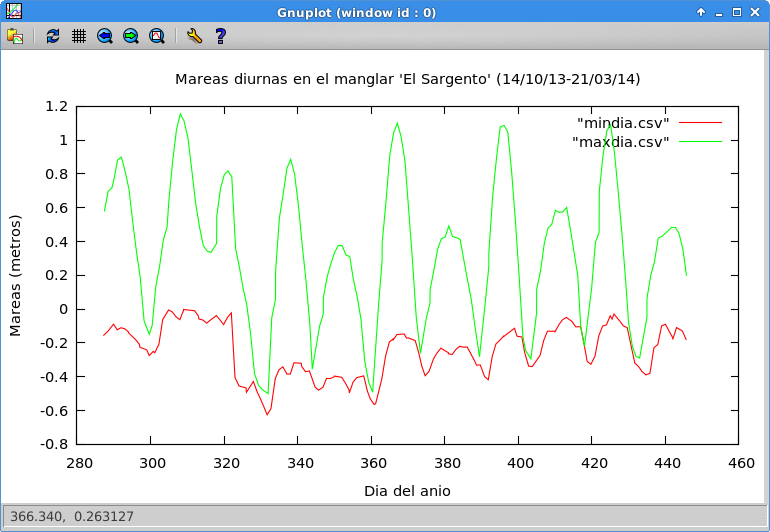
\includegraphics[scale=0.6]{maxymindias.png} 
\end{center}

\begin{large}
Mareas semidiurnas.\\
Al encontrar los maximos y minimos en lapsos de 12 horas fue posible encontrar el periodo promedio de las mareas semidiurnas en el manglar El Sargento, encontrando que el periodo es de 0.4992 dias, o bien 11 horas y 58 minutos.
\end{large}

\begin{center}
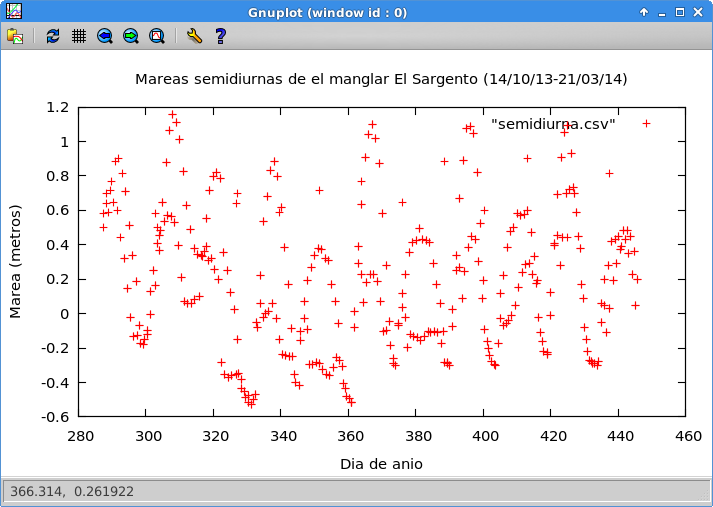
\includegraphics[scale=0.8]{semidiurnas.png} 
\end{center}

\begin{large}
Mareas de ciclo lunar.\\
Estas corresponden a buscar máximos y mínimos en lapsos de un mes, es decir, cada 28 días. De este análisis de encontro un periodo promedio lunar de 29.25 días, es decir 29 dias y 6 horas.

\begin{center}
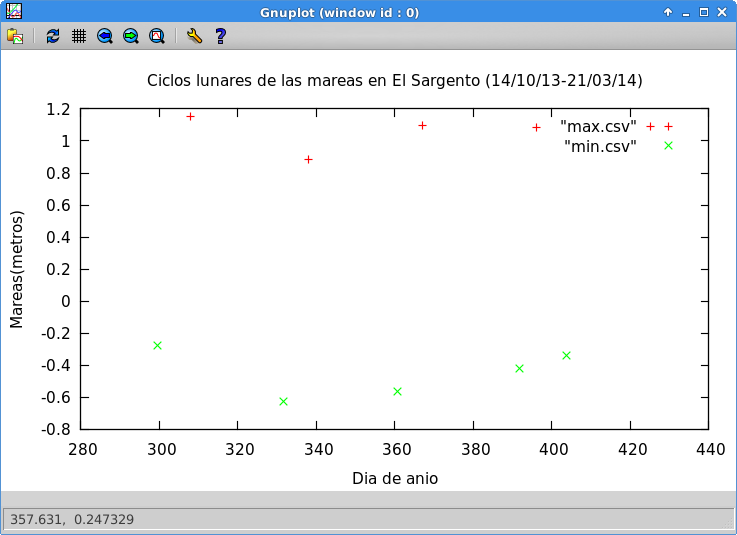
\includegraphics[scale=0.8]{Sin_nombre.png} 
\end{center}

Finalmente, de esta actividad podemos concluir la forma en que afectan las posiciones del Sol y la Luna en las mareas, ya que ,por ejemplo, la marea diurna nos indica que existe cierta posición del Sol que ocasiona la máxima marea de un dia, y obviamente no vuelve a estar en esa posición si no hasta un día después, es por eso que el periodo es de casi 24 horas.\\
De igual modo, el ciclo lunar nos señala esa posicion de la Luna que afecta mas favorablemente a las mareas, marcando asi un periodo de casi 29 dias, el cual coincide con el periodo en que se presenta una Luna llena.\\
Analizando los datos de esta forma, es sencillo darse cuenta la forma en que los astros afectas a los mares.

\end{large}

\newpage
\begin{center}
\begin{LARGE}
Código.
\end{LARGE}
\end{center}
\begin{verbatim}
Module periodos
implicit none
integer, parameter :: datos=7632, mes=1344, dias=159, dia=48, mediodia=24, 
mesesc=5376!datos en los meses completos
end module periodos

Program Mareas
use periodos
Implicit None
real :: p, t, d, mx, im, maximo, minimo, minimod, maximod, maximd
real, dimension(1:datos):: B, altura, tiempo, tiem, maxm, min
real, dimension(1:5):: mm, tm, periodomaxm,  periodominm
real, dimension(1:dias)::  periodomaxd, periodomind
real, dimension(1:318):: periodomd
integer :: i, j

open(unit=8, file='Mareas.csv',status='old')
do i=1, datos, 1 
   read (8,*) B(i), p, t, altura(i), d, tiempo(i)
  !write (*,*) B(i),p, t, altura(i), d, tiempo(i)
end do  

print * , '-------------------------------'
print * , 'Niveles máximos por mes'
open(unit=10, file='max.csv', status='unknown')
do j=0, mesesc, mes
maximo = -1
  do i=1,mes,1
     if(altura(i+j).gt.maximo) then
     maximo = altura(i+j)
     mx = tiempo(i+j)
     end if
     continue
  end do
      write(10,*) mx, maximo
     ! write(*,*) mx, maximo
end do  
close(10)

print * , 
print * , '-------------------------------'
print * , 'Niveles minimos por mes'
open(unit=11,file='min.csv',status='unknown')

do j=0, mesesc, mes
minimo=0
  do i=1,mes,1
   if(altura(i+j).lt.minimo) then
   minimo = altura(i+j)
   im = tiempo(i+j)
   end if
  end do
  write(11,*) im, minimo
   !write(*,*) im, minimo
end do
close(11)

print * , '--------------------------------'
print * , '!Mínimos diarios'
open (unit=12, file='mindia.csv', status='unknown')
do j=0,datos-1,dia
minimod=0
  do i=1,dia,1
  if(altura(i+j).lt.minimod) then
  minimod = altura(i+j)
  im = tiempo(i+j) 
  end if
  end do
  write (12,*) im, minimod
  !write (*,*) im, minimod
end do
close(12)

print * , '--------------------------------'
print * ,'!Máximos diarios'
open (unit=13, file='maxdia.csv', status='unknown')
do j=0,datos-1,dia
maximod=-1
  do i=1,dia,1
  if(altura(i+j).gt.maximod) then
  maximod = altura(i+j)
  im = tiempo(i+j)
  end if
  end do
  write (13,*) im, maximod
 !write (*,*) im, maximod
end do
close(13)
close (8)

print * , 'nivel de marea máxima', maximo
print * , 'mivel de marea mímina', minimo
print * , 'tiempo de marea mínima', dia

print * , '-------------------------------'
print * , 'Periodos entre máximos por mes'
open(unit=10, file='max.csv', status='unknown')
do i=1,5, 1
   read(10,*) tm(i), mm(i)
 if (i .gt. 1) then
   periodomaxm(i) = tm(i) - tm(i-1)
 end if
   !write(*,*) periodomaxm(i)
  
end do
  !write(*,*) periodomaxm
  print * , 'Periodo promedio entre maximos mensuales'
  write(*,*) sum(periodomaxm)/4, 'dias'
close(10)

print * , '-------------------------------'
print * , 'Periodos entre mínimos por mes'
open(unit=11,file='min.csv',status='unknown')
do i=1,5,1
  read(11,*) tm(i), mm(i)
  periodominm(i) = tm(i) - tm(i-1)
  !write(*,*) periodominm(i)
end do
  !write(*,*) periodominm(i)
close(11)

print * , '-------------------------------'
print * , 'Periodos entre mínimos por dias'
open (unit=12, file='mindia.csv', status='unknown')
do i =1,159,1
   read(12,*) tm(i), mm(i)
   periodomind(i) = tm(i) - tm(i-1)
  !write(*,*) periodomind(i)
end do
  !write(*,*) periodomind(i)
close(12)

print * , '-------------------------------'
print * , 'Periodos entre máximos por dias'
open (unit=13, file='maxdia.csv', status='unknown')
do i=1,dias,1
   read(13,*) tm(i), mm(i)
if (i .gt. 1) then
   periodomaxd(i) = tm(i)-tm(i-1)
end if
   !write(*,*) periodomaxd(i)
end do
   print * , '-------------------------------'
   print * , 'Periodo promedio entre maximos diarios'
  !write(*,*) sum(periodomaxd)/(dias-1), 'dias'
close(13)

print * , '-------------------------------'
print * , 'mareas semidiurnas'
open(unit=8, file='Mareas.csv',status='old')
do i=1, datos, 1 
   read (8,*) B(i), p, t, altura(i), d, tiempo(i)
  !write (*,*) B(i),p, t, altura(i), d, tiempo(i)
end do  

open (unit=14, file='semidiurna.csv', status='unknown')
do i=1,318,1
   read(14,*) tm(i),mm(i)
end do

do j=0,datos-1,mediodia
 maximd=-1
 do i=1,mediodia,1
  if(altura(i+j).gt.maximd) then
  maximd = altura(i+j)
  im = tiempo(i+j)
  end if
 end do 
  write (14,*) im, maximd
  !write (*,*) im, maximd
end do

print * , '-------------------------------'
print * , 'diferencias entre mareas semidiurnas'
!promedio semidiurnas
do i=1,318,1
  if (i .gt. 1) then
   periodomd(i) = tm(i)-tm(i-1)
  end if
  write(*,*) periodomd(i)
end do
   print * , '-------------------------------'
   print * , 'Periodo promedio entre mareas semidiurnas'
  write(*,*) sum(periodomd)/317, 'dias' 
close(14)
close(8)

end Program Mareas




\end{verbatim}

\end{document}


